% Created by tikzDevice version 0.12.3.1 on 2021-11-10 17:09:39
% !TEX encoding = UTF-8 Unicode
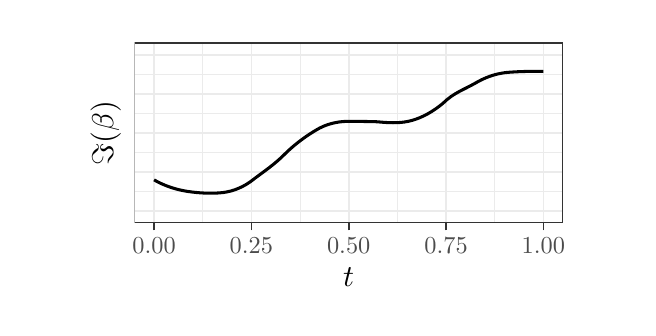
\begin{tikzpicture}[x=1pt,y=1pt]
\definecolor{fillColor}{RGB}{255,255,255}
\path[use as bounding box,fill=fillColor,fill opacity=0.00] (0,0) rectangle (216.81,101.18);
\begin{scope}
\path[clip] ( 17.93,  0.00) rectangle (198.88,101.18);
\definecolor{drawColor}{RGB}{255,255,255}
\definecolor{fillColor}{RGB}{255,255,255}

\path[draw=drawColor,line width= 0.6pt,line join=round,line cap=round,fill=fillColor] ( 17.93,  0.00) rectangle (198.88,101.18);
\end{scope}
\begin{scope}
\path[clip] ( 38.64, 30.69) rectangle (193.38, 95.68);
\definecolor{fillColor}{RGB}{255,255,255}

\path[fill=fillColor] ( 38.64, 30.69) rectangle (193.38, 95.68);
\definecolor{drawColor}{gray}{0.92}

\path[draw=drawColor,line width= 0.3pt,line join=round] ( 38.64, 42.08) --
	(193.38, 42.08);

\path[draw=drawColor,line width= 0.3pt,line join=round] ( 38.64, 56.15) --
	(193.38, 56.15);

\path[draw=drawColor,line width= 0.3pt,line join=round] ( 38.64, 70.22) --
	(193.38, 70.22);

\path[draw=drawColor,line width= 0.3pt,line join=round] ( 38.64, 84.28) --
	(193.38, 84.28);

\path[draw=drawColor,line width= 0.3pt,line join=round] ( 63.26, 30.69) --
	( 63.26, 95.68);

\path[draw=drawColor,line width= 0.3pt,line join=round] ( 98.43, 30.69) --
	( 98.43, 95.68);

\path[draw=drawColor,line width= 0.3pt,line join=round] (133.60, 30.69) --
	(133.60, 95.68);

\path[draw=drawColor,line width= 0.3pt,line join=round] (168.77, 30.69) --
	(168.77, 95.68);

\path[draw=drawColor,line width= 0.6pt,line join=round] ( 38.64, 35.05) --
	(193.38, 35.05);

\path[draw=drawColor,line width= 0.6pt,line join=round] ( 38.64, 49.11) --
	(193.38, 49.11);

\path[draw=drawColor,line width= 0.6pt,line join=round] ( 38.64, 63.18) --
	(193.38, 63.18);

\path[draw=drawColor,line width= 0.6pt,line join=round] ( 38.64, 77.25) --
	(193.38, 77.25);

\path[draw=drawColor,line width= 0.6pt,line join=round] ( 38.64, 91.32) --
	(193.38, 91.32);

\path[draw=drawColor,line width= 0.6pt,line join=round] ( 45.67, 30.69) --
	( 45.67, 95.68);

\path[draw=drawColor,line width= 0.6pt,line join=round] ( 80.84, 30.69) --
	( 80.84, 95.68);

\path[draw=drawColor,line width= 0.6pt,line join=round] (116.01, 30.69) --
	(116.01, 95.68);

\path[draw=drawColor,line width= 0.6pt,line join=round] (151.18, 30.69) --
	(151.18, 95.68);

\path[draw=drawColor,line width= 0.6pt,line join=round] (186.35, 30.69) --
	(186.35, 95.68);
\definecolor{drawColor}{RGB}{0,0,0}

\path[draw=drawColor,line width= 1.1pt,line join=round] ( 45.67, 46.17) --
	( 47.07, 45.42) --
	( 48.46, 44.75) --
	( 49.85, 44.16) --
	( 51.25, 43.64) --
	( 52.64, 43.18) --
	( 54.03, 42.79) --
	( 55.42, 42.45) --
	( 56.82, 42.17) --
	( 58.21, 41.95) --
	( 59.60, 41.77) --
	( 61.00, 41.62) --
	( 62.39, 41.50) --
	( 63.78, 41.42) --
	( 65.17, 41.37) --
	( 66.57, 41.37) --
	( 67.96, 41.40) --
	( 69.35, 41.48) --
	( 70.75, 41.62) --
	( 72.14, 41.86) --
	( 73.53, 42.19) --
	( 74.92, 42.63) --
	( 76.32, 43.18) --
	( 77.71, 43.83) --
	( 79.10, 44.61) --
	( 80.50, 45.53) --
	( 81.89, 46.59) --
	( 83.28, 47.63) --
	( 84.67, 48.65) --
	( 86.07, 49.69) --
	( 87.46, 50.74) --
	( 88.85, 51.84) --
	( 90.24, 53.01) --
	( 91.64, 54.26) --
	( 93.03, 55.62) --
	( 94.42, 56.94) --
	( 95.82, 58.18) --
	( 97.21, 59.33) --
	( 98.60, 60.41) --
	( 99.99, 61.43) --
	(101.39, 62.39) --
	(102.78, 63.29) --
	(104.17, 64.15) --
	(105.57, 64.93) --
	(106.96, 65.58) --
	(108.35, 66.11) --
	(109.74, 66.53) --
	(111.14, 66.86) --
	(112.53, 67.10) --
	(113.92, 67.25) --
	(115.32, 67.33) --
	(116.71, 67.34) --
	(118.10, 67.34) --
	(119.49, 67.31) --
	(120.89, 67.29) --
	(122.28, 67.27) --
	(123.67, 67.26) --
	(125.07, 67.23) --
	(126.46, 67.16) --
	(127.85, 67.04) --
	(129.24, 66.93) --
	(130.64, 66.86) --
	(132.03, 66.83) --
	(133.42, 66.85) --
	(134.82, 66.94) --
	(136.21, 67.10) --
	(137.60, 67.35) --
	(138.99, 67.70) --
	(140.39, 68.15) --
	(141.78, 68.69) --
	(143.17, 69.33) --
	(144.57, 70.05) --
	(145.96, 70.87) --
	(147.35, 71.78) --
	(148.74, 72.79) --
	(150.14, 73.92) --
	(151.53, 75.18) --
	(152.92, 76.25) --
	(154.31, 77.17) --
	(155.71, 77.97) --
	(157.10, 78.71) --
	(158.49, 79.41) --
	(159.89, 80.13) --
	(161.28, 80.87) --
	(162.67, 81.65) --
	(164.06, 82.38) --
	(165.46, 83.01) --
	(166.85, 83.56) --
	(168.24, 84.02) --
	(169.64, 84.40) --
	(171.03, 84.69) --
	(172.42, 84.92) --
	(173.81, 85.06) --
	(175.21, 85.15) --
	(176.60, 85.23) --
	(177.99, 85.29) --
	(179.39, 85.34) --
	(180.78, 85.37) --
	(182.17, 85.39) --
	(183.56, 85.39) --
	(184.96, 85.38) --
	(186.35, 85.38);
\definecolor{drawColor}{gray}{0.20}

\path[draw=drawColor,line width= 0.6pt,line join=round,line cap=round] ( 38.64, 30.69) rectangle (193.38, 95.68);
\end{scope}
\begin{scope}
\path[clip] (  0.00,  0.00) rectangle (216.81,101.18);
\definecolor{drawColor}{gray}{0.20}

\path[draw=drawColor,line width= 0.6pt,line join=round] ( 45.67, 27.94) --
	( 45.67, 30.69);

\path[draw=drawColor,line width= 0.6pt,line join=round] ( 80.84, 27.94) --
	( 80.84, 30.69);

\path[draw=drawColor,line width= 0.6pt,line join=round] (116.01, 27.94) --
	(116.01, 30.69);

\path[draw=drawColor,line width= 0.6pt,line join=round] (151.18, 27.94) --
	(151.18, 30.69);

\path[draw=drawColor,line width= 0.6pt,line join=round] (186.35, 27.94) --
	(186.35, 30.69);
\end{scope}
\begin{scope}
\path[clip] (  0.00,  0.00) rectangle (216.81,101.18);
\definecolor{drawColor}{gray}{0.30}

\node[text=drawColor,anchor=base,inner sep=0pt, outer sep=0pt, scale=  0.88] at ( 45.67, 19.68) {0.00};

\node[text=drawColor,anchor=base,inner sep=0pt, outer sep=0pt, scale=  0.88] at ( 80.84, 19.68) {0.25};

\node[text=drawColor,anchor=base,inner sep=0pt, outer sep=0pt, scale=  0.88] at (116.01, 19.68) {0.50};

\node[text=drawColor,anchor=base,inner sep=0pt, outer sep=0pt, scale=  0.88] at (151.18, 19.68) {0.75};

\node[text=drawColor,anchor=base,inner sep=0pt, outer sep=0pt, scale=  0.88] at (186.35, 19.68) {1.00};
\end{scope}
\begin{scope}
\path[clip] (  0.00,  0.00) rectangle (216.81,101.18);
\definecolor{drawColor}{RGB}{0,0,0}

\node[text=drawColor,anchor=base,inner sep=0pt, outer sep=0pt, scale=  1.10] at (116.01,  7.64) {$t$};
\end{scope}
\begin{scope}
\path[clip] (  0.00,  0.00) rectangle (216.81,101.18);
\definecolor{drawColor}{RGB}{0,0,0}

\node[text=drawColor,rotate= 90.00,anchor=base,inner sep=0pt, outer sep=0pt, scale=  1.10] at ( 31.00, 63.18) {$\Im(\beta)$};
\end{scope}
\end{tikzpicture}
